\part{SW 02 - ISO/OSI Modell}
\section{Lernziele (Leitfragen)}
\begin{enumerate}
    \item Was sind die Schichten des TCP/IP Models? Beschreiben Sie den Zweck jeder Schicht
    \item Was sind die Schichten des OSI Models? Beschreiben Sie den Zweck jeder Schicht
    \item Was ist die Verbindung zwischen dem TCP/IP Modell und dem OSI Modell?
    \item Nehmen Sie eine typische Netzwerkapplikation als Beispiel. Anhand des TCP/IP Models, erläutern Sie wie Nachrichten zwischen den End-Devices ausgetauscht sind.
    \item Wieso muss man Zahlensysteme verstehen, wenn man sich mit Computernetzwerken beschäftigt?
    \item Wie kann man einfach und schnell zwischen Binär, Hexadezimal und Dezimal umrechnen?
\end{enumerate}

\section{Antworten}
\subsection*{Was sind die Schichten des TCP/IP Models? Beschreiben Sie den Zweck jeder Schicht}\index{Modell!TCP/IP}
Das TCP/IP Modell besteht aus vier Schichten.\\
Eselsbrücke: \underline{$\mathbb{A}$}lle \underline{$\mathbb{T}$}iere \underline{$\mathbb{I}$}n \underline{$\mathbb{N}$}oah's \underline{$\mathbb{A}$}rche\\

\begin{table}[H]
\begin{tabularx}{\textwidth}{|c|X|l|}
    \multicolumn{1}{c}{Layer}&\multicolumn{1}{X}{Zusammenfassung}&\multicolumn{1}{l}{Protokolle}\\
    \hline
    \makecell[c]{Application}&\makecell[X]{- Am nächsten zum User\\- Datenaustausch zwischen Programmen\\- Allgemeine Funktionen zur Kommunikation im Internet}&\makecell[l]{Web (HTTP, HTTPS)\\Email (POP, IMAP, SMTP)\\Namensauflösung (DNS)\\Datenaustausch (FTP)}\\
    \hline
    \makecell{Transport}&\makecell[X]{- Segmentierung und Zusammenfügen von Daten\\- Management von Verlässlichkeitsanforderungen einer Konversation\\- Multiplexing und Konversationen verfolgen}&\makecell[l]{Verbindungsorierntiert (TCP)\\Verbindungslos (UDP)}\\
    \hline
    \makecell{Internet}&\makecell[X]{- Datenaustausch über Sub-Netzwerke\\- Adressierung von Endgeräten\\- Routing\\- verbindungslos, best effort und medienunabhängig}&\makecell[l]{Datenaustausch (IPv4, IPv6)\\Routing (OSPF, BGP)\\Steuerung (ICMPv4, ICMPv6)}\\
    \hline
    \makecell{Network\\Access}&\makecell[X]{- Adressierung von Sub-Netzwerken\\- Media access control (MAC)\\- Abstraktion der physischen Medien der oberen Schichten\\- Bits auf die Medien setzen}&\makecell[l]{Address Resolution (ARP)\\Data Link (Ethernet, WLAN)}\\
    \hline
\end{tabularx}
\caption{TCP/IP Modell}
\end{table}

\subsection*{Was sind die Schichten des OSI Models? Beschreiben Sie den Zweck jeder Schicht}\index{Modell!OSI}\label{sub:SchichtenOSIModell}
Das OSI Modell besteht aus 7 Schichten.\\
Eselsbrücke: \underline{$\mathbb{A}$}lle \underline{$\mathbb{P}$}riester \underline{$\mathbb{S}$}aufen \underline{$\mathbb{T}$}equilla \underline{$\mathbb{N}$}ach \underline{$\mathbb{D}$}er \underline{$\mathbb{P}$}redigt\\

\begin{table}[H]
\begin{tabularx}{\textwidth}{|c|X|c|}
    \multicolumn{1}{c}{Layer}&\multicolumn{1}{X}{Zusammenfassung}&\multicolumn{1}{l}{Protokolle}\\
    \hline
    \multicolumn{3}{|c|}{$\downarrow$Anwendungsorientiert$\downarrow$}\\
    \hline
    \makecell[c]{Layer VII\\Anwendungen\\(Application)}&\makecell[X]{Die Anwendungsschicht interagiert direkt mit der Software (Anwendung), die eine Netzwerkübertragung anfordert. Sie ermittelt, ob die Möglichkeit einer Verbindung besteht, und identifiziert und sucht Ressourcen.}&\multirow{12}{*}{\makecell[c]{DHCP\\DNS\\FTP\\HTTPS\\LDAP\\SMTP\\\dots}}\\
    \cline{1-2}

    \makecell[c]{Layer VI\\Darstellung\\(Presentation)}&\makecell[X]{Die Darstellungsschicht sorgt dafür, dass die Daten so bearbeitet werden, dass sie optimal ausgetauscht und verarbeitet werden können. Hierfür gibt es etliche standardisierte Kodierungs-, Konvertierungs- und Kompressionsverfahren, zum Beispiel für Verschlüsselungsroutinen, Zeichendarstellungen, Video- und Audioübertragungen.}&\\
    \cline{1-2}

    \makecell[c]{Layer V\\Kommunikations-/\\Sitzungsschicht\\(Session)}&\makecell[X]{Die Kommunikationsschicht ist hauptsächlich eine `'Serviceschicht'' für die bidirektionale Kommunikation von Anwendungen in verschiedenen Endgeräten. Sitzungen und Datenströme werden angefordert, aufgebaut, kontrolliert und koordiniert. Meist bedienen sich die Services der Schicht 5 dabei der Dienstangebote der Schicht 4.}&\\
    \hline

    \makecell[c]{Layer IV\\Transportschicht\\(Transport)}&\makecell[X]{In der Transportschicht sind Sicherungsmechanismen für einen zuverlässigen Datentransport beschrieben. Die Schicht 4 regelt das Datenmultiplexing und die Flusskontrolle, das heisst, mehrere Anwendungen höherer Protokolle können gleichzeitig Daten über eine Verbingdung tranportieren. In der Tranportschicht sind verbindugslose und verbindungsorientierte Dienste implementiret. Verbindungsorientierte Diense können einen sehr sicheren Datenaustausch durchführen. Der Sender und der Empfänger kontrollieren ihre Möglickeiten der Kommunikation (Aufbau einer virtuellen Verbindung), die Daten werden erst nach dieser Prfung versandt. Eine weitgehende Fehlerkontrolle prüft die Daten und fordert entweder verlorene oder korrumpierte Daten zur erneuten Übersendung an. Am Ende der Kommunikation wird die Verbindung gezielt und kontrolliert wieder abgebaut. Im Layer 4 wird nach definierten Anwendungen unterschieden. Hier beginnt die Kommunikation zwischen dem Netzwerk un der Anwendung.}&\makecell[c]{TCP\\UDP\\\dots}\\
    \hline

    \multicolumn{3}{|c|}{$\downarrow$Transportorientiert$\downarrow$}\\
    \hline

    \makecell[c]{Layer III\\Vermittlungsschicht\\(Network)}&\makecell[X]{In der Schicht 3 des OSI-Modells wird die logische Adressierung (segmentübergreifend bis weltweit) der Geräte definiert. Die Routing-Protokolle dieser Schicht ermöglichen die Wegfindung in grossen (bis weltweiten) Netzwerken und redundante Wege ohne Konflikte. Routing-Protokolle sorgen ebenfalls dafür, dass die Ressourcen in vermaschten Netzen mit vielen redundanten Wegen bei dem Ausfall einer Verbindung weiterhin benutzt werden können.}&\makecell[c]{ICMP\\IP\\IPsec\\IPX\\\dots}\\
    \hline

    \makecell[c]{Layer II\\Sicherungsschicht\\(Data Link)}&\makecell[X]{Die Sicherungsschicht ist für eine zuverlässige Übertragung der Daten zuständig. Sie regelt die Flusssteuerung, regelt den Zugriff, verhindert eine Überlastung des Empfängers und ist für die physikalische Adressierung innerhalb eines Netzsegmentes auf dieser Schicht verantwortlich. Hier ist die erste Fehlererkennung implementiert. Die Topologie eines Netzwerkes ist stark von dieser Schicht abhängig, sie definiert die Art und Weise, wie die Rechner und Netzwerkgeräte miteinander verbunden sind.}&\makecell[c]{IEEE 802.3\\(Ethernet)\\IEEE 802.11\\(WLAN)\\MAC\\\dots}\\
    \hline

    \makecell[c]{Layer I\\Physikalische Schicht\\(Physical)}&\makecell[X]{Hier sind die physikalischen Parameter definiert. Dazu gehören Kapeltypen, die Anschlüsse, die Streckenlängen, die elektrischen Eckdaten wie Spannungen, Frequenzen etc. Getrennt wird hier in drei Bereiche:\\\begin{itemize}
        \item Der Nahbereich (LAN)
        \item mittlere Entfernungen (MAN)
        \item und Fernverbindungen (WAN).
    \end{itemize}}&\makecell[c]{1000BASE-T\\10BASE-T\\Token Ring\\\dots}\\
    \hline

\end{tabularx}
\caption{OSI Modell\cite{Schreiner2019}}
\end{table}
\subsection*{Was ist die Verbindung zwischen dem TCP/IP Modell und dem OSI Modell?}\label{sub:VerbindungTCPundOSIModell}
\begin{figure}[H]
    \begin{center}
    \label{pic:osi_tcpip}
    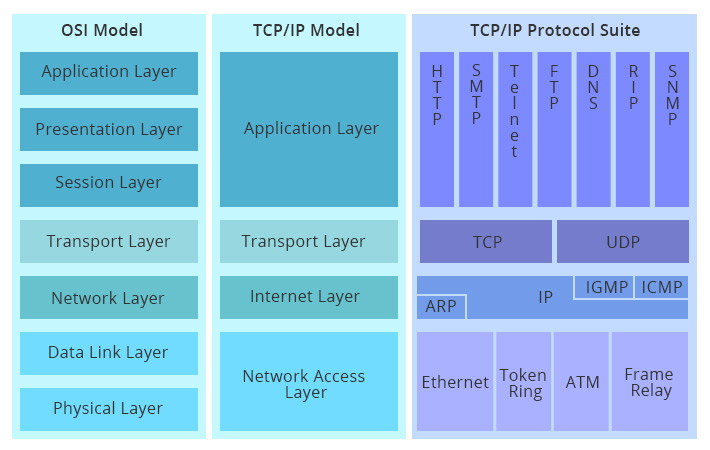
\includegraphics[width=\textwidth]{images/osi_tcpip.jpg}
    \caption[Vergleich OSI mit TCP/IP Modell]{Vergleich OSI mit TCP/IP Modell\cite{FSDeutschland}}
    \end{center}
\end{figure}

\subsection*{Nehmen Sie eine typische Netzwerkapplikation als Beispiel. Anhand des TCP/IP Models, erläutern Sie wie Nachrichten zwischen den End-Devices ausgetauscht sind.}\label{sub:BeispielNetzwerkapplikation}
\begin{figure}[H]
    \begin{center}
    \label{pic:tcp1}
    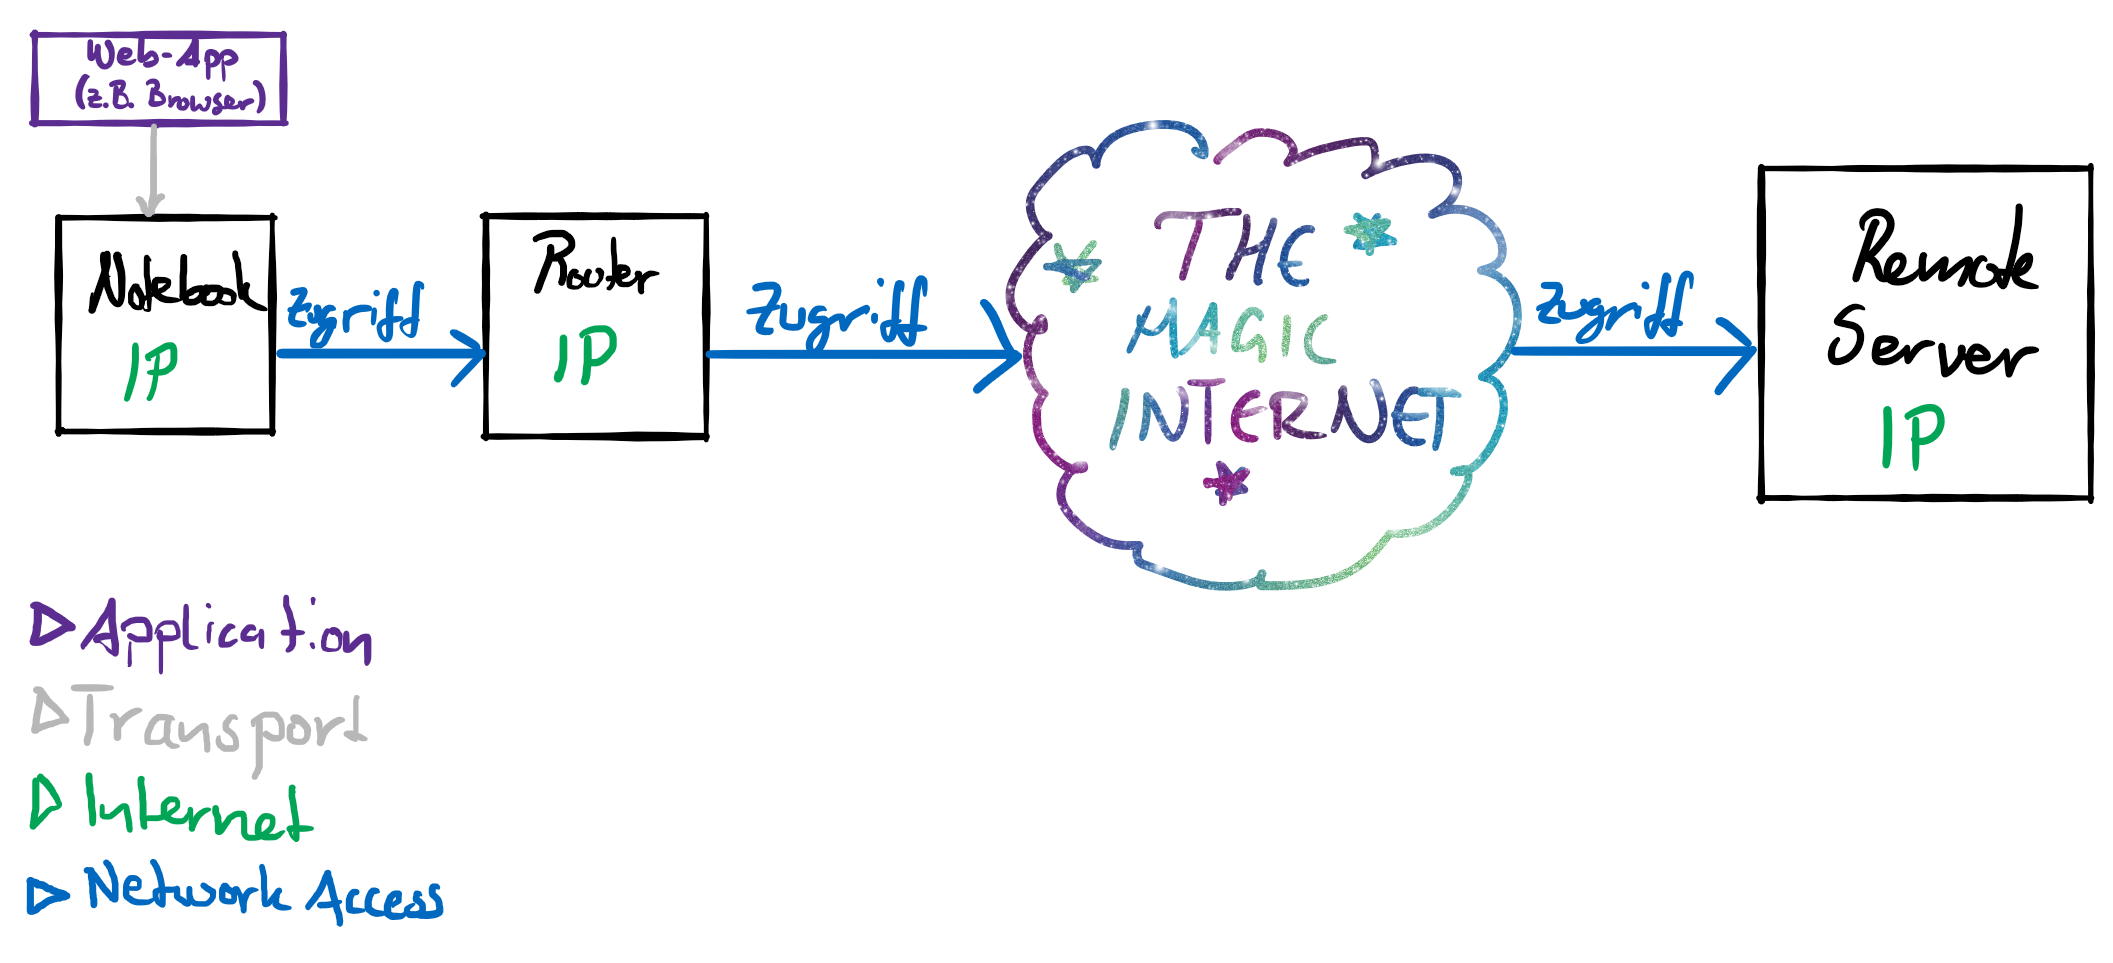
\includegraphics[width=\textwidth]{images/Nachrichtenaustausch01.png}
    \caption{Weg eines Datenpaketes}
    \end{center}
\end{figure}

\begin{figure}[H]
    \begin{center}
    \label{pic:tcp2}
    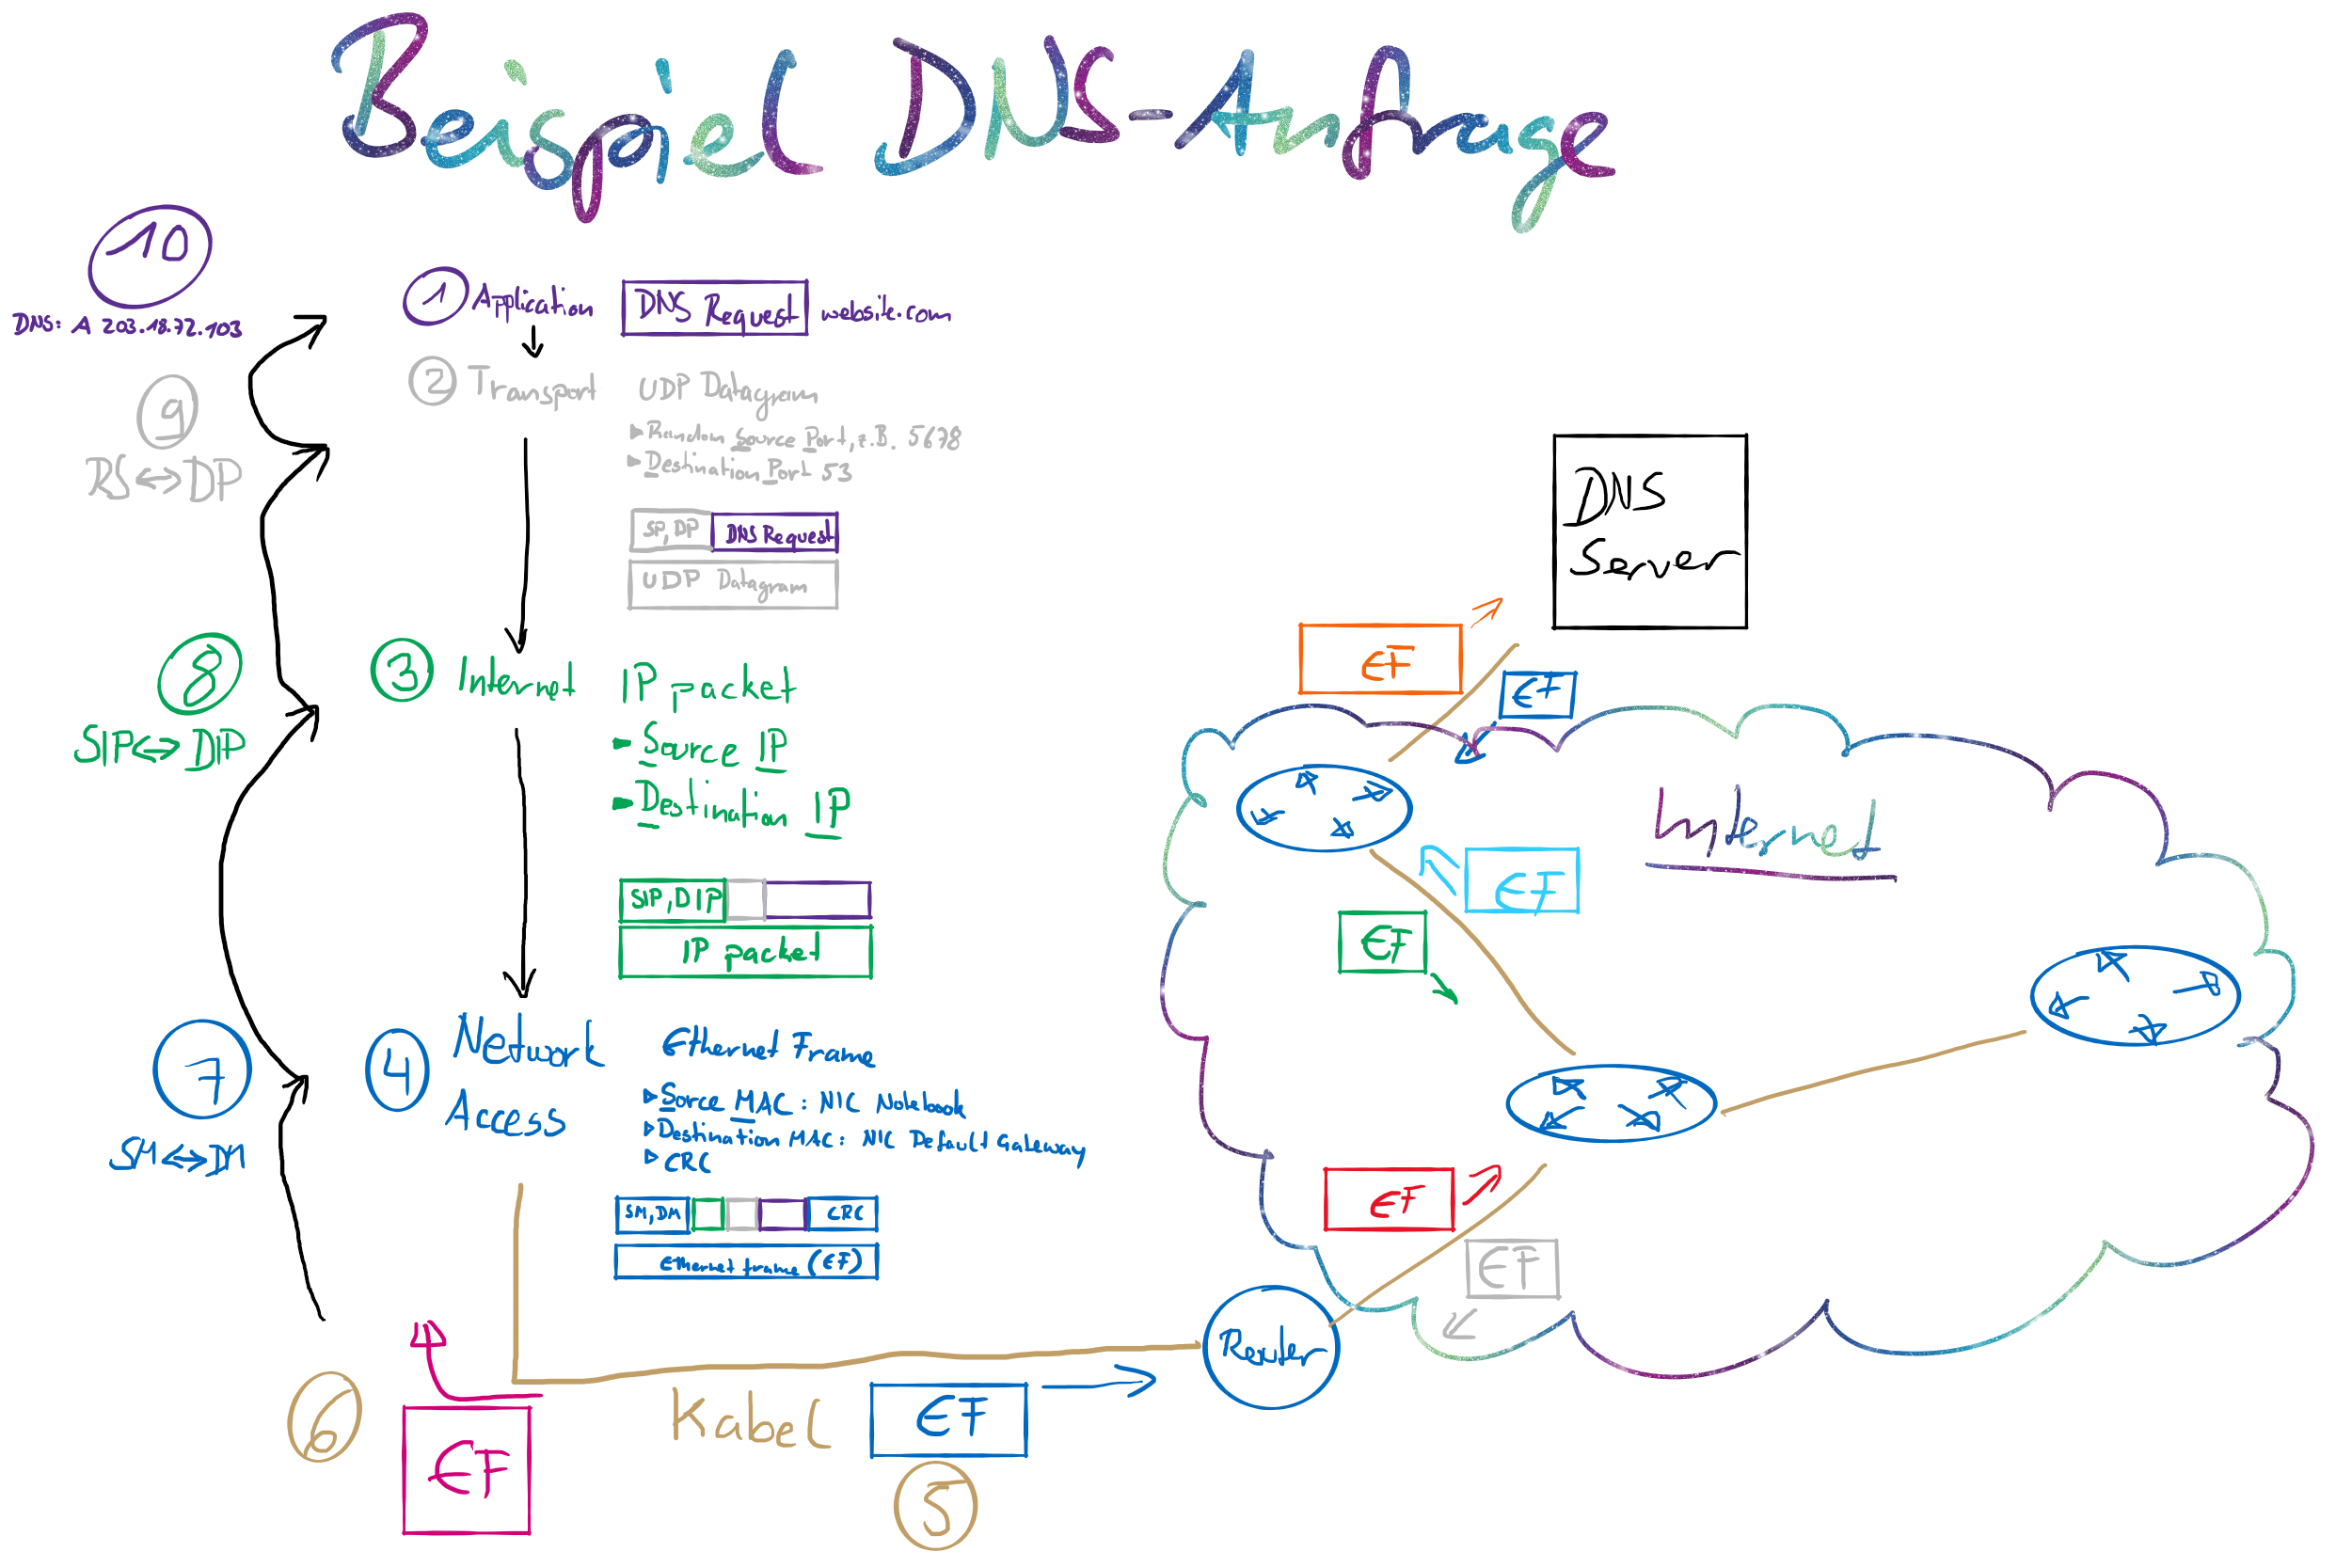
\includegraphics[width=\textwidth]{images/Nachrichtenaustausch02.png}
    \caption{Einzelschritte der Kapselung, Beispiel anhand DNS request}
    \end{center}
\end{figure}

\subsection*{Wieso muss man Zahlensysteme verstehen, wenn man sich mit Computernetzwerken beschäftigt?}\label{sub:ZahlensystemeVerstehen}
Das Rechnen mit anderen Zahlensystemen wie Binär ist im Umgang mit Computernetzwerken insofern wichtig, weil gewisse Rechnungen (z.B. Subnetz) einfacher sind. Auch sind gewisse Zahlen in anderen Formaten dargestellt wie MAC-Adressen oder IPv6, welche in Hexadezimal dargestellt werden, weil diese kompakter sind als Dezimal.

\pagebreak
\subsection*{Wie kann man einfach und schnell zwischen Binär, Hexadezimal und Dezimal umrechnen?}\label{sub:RechnenBinHexDez}
    Über den Rechner vom Betriebssystem:
    \begin{figure}[H]
        \begin{center}
        \label{pic:calc}
        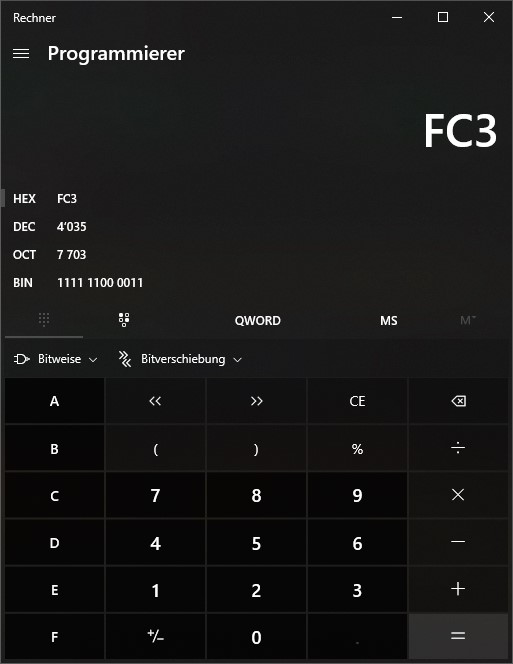
\includegraphics[width=.5\textwidth]{images/calc.jpg}
        \caption{Windows Taschenrechner}
        \end{center}
    \end{figure}
    Oder ganz easy von Hand ausrechnen.
    \paragraph{Binär}Beispiel $125_{10}$ zu Binär. Den Rest zusammenfügen:\\
    \begin{tabular}{rcll}
        125&$\div$&2 = 62&R 1 (ganz rechts)\\
        62&$\div$&2 = 31&R 0\\
        31&$\div$&2 = 15&R 1\\
        15&$\div$&2 = 7&R 1\\
        7&$\div$&2 = 3&R 1\\
        3&$\div$&2 = 1&R 1\\
        1&$\div$&2 = 0&R 1 (ganz links)\\[1em]
\end{tabular}
Dann ist das Ergebnis also: 0b111 1101\\[1em]
Um die Binärzahl in Dezimal umzuwandeln, liest man von rechts die Einsen und fängt mit der Potenz 0 zur Basis 2 an. Unser Zahlenbeispiel als Byte:\\[1em]
\begin{tabular}{cccccccc}
    $2^7$&$2^6$&$2^5$&$2^4$&$2^3$&$2^2$&$2^1$&$2^0$\\
    0&1&1&1&1&1&0&1\\
\end{tabular}\\[1em]
Daraus erhält man, dort wo eine 1 steht:\\$2^6+2^5+2^4+2^3+2^2+2^0=64+32+16+8+4+1=125$.

\pagebreak
\paragraph{Hexadezimal}Hexadezimal ist da schon etwas komplizierter, aber machbar. Hier rechnet man auch mit Potenzen zur Basis 16. Dazu muss man vorgängig aber schon das $16^x$ unterhalb der Zahl kennen.\\
$16^2=256$ ist also zu hoch für unsere 125. Bleibt also die nächst tiefere Potenz  $16^1=16$.\\
Wir teilen also mit 16:\\
\begin{tabular}{rcllll}
    125&$\div$&16&($16^1$)&= 7 (ganz links)&R  13 (mit nächst tiefere Potenz teilen)\\
    13&$\div$&1&($16^0$) &= 13&\\[1em]
\end{tabular}\\
Also hat man jetzt $7\times16^1+13\times16^0$. Das Hexadezimalsystem geht ja aber von 0-F, somit ist die 13 ein D (\dots, 9, 10=A, 11=B, 12=C, 13=D, 14=E, 15=F). Das Ergebnis ist als 0x7D. Auch easy.\\
Umgekehrt von Hexadezimal auf Dezimal umzurechnen, folgt man dem nun bekannten Potenz-Prinzip.\\
Hexadezimal und Binär ist Bubieinfach. Dazu nimmt man Binär halbe Bytes und stellt die Zahlen gegenüber.\\
\begin{tabular}{cccc|cccc}
    $2^3$&$2^2$&$2^1$&$2^0$&$2^3$&$2^2$&$2^1$&$2^0$\\
    0&1&1&1&1&1&0&1\\
    \hline
    \multicolumn{4}{c|}{7}&\multicolumn{4}{c}{13 = D}\\
\end{tabular}\\[1em]

Was ist mit grossen Zahlen? Dazu brauchen wir einen Taschenrechner mit der Log-Funktion. Nehmen wir als Beispiel $1'106'132_{10}$. Um die Potenz $x$ von $16^x$ herauszufinden, logarithmieren wir diese Zahl mit dem Taschenrechner: $\frac{\log{1106132}}{\log{16}}=5.00000103189442\dots$ \\
Wir wissen nun, das es sich beim Exponenten um die Potenz 5 handelt. Teilen die Zahl mit $16^5$ und erhalten $1.0548\dots$ Wir subtrahieren die 1 vom Ergebnis und die Nachkommastellen$\times$\underline{Divisor} (hier $16^5$) ergeben den Rest von 57556. Den Rest wieder logarithmieren für nächste Potenz u.s.w. Wir rechnen nun (Zwischenschritt für Rest und Potenz nicht dabei):\\
\begin{tabular}{rcllll}
    1106132&$\div$&1048576&($16^5$)&= 1 (ganz links)&R 57556 (mit nächst tiefere Potenz teilen)\\
    57556&$\div$&4096&($16^3$)&= 14&R 212\\
    212&$\div$&16&($16^1$)&= 13&R 4\\
    4&$\div$&1&$(16^0)$&= 4&R 0\\[1em]
\end{tabular}\\

Nun können wir überall dort, wo ein Exponent steht, die Zahl Schreiben. Überall dort wo kein Exponent ist (hier: 4, 2), wird 0 geschrieben:\\
\begin{tabular}{cccc|c|cccc|c|cccc|cccc}
    $2^3$&$2^2$&$2^1$&$2^0$&&$2^3$&$2^2$&$2^1$&$2^0$&&$2^3$&$2^2$&$2^1$&$2^0$&$2^3$&$2^2$&$2^1$&$2^0$\\
    0&0&0&1&0000&1&1&1&0&0000&1&1&0&1&0&1&0&0\\
    \hline
    \multicolumn{4}{c|}{1}&\multicolumn{1}{c|}{0}&\multicolumn{4}{c|}{14 = E}&\multicolumn{1}{c|}{0}&\multicolumn{4}{c|}{13 = D}&\multicolumn{4}{c}{4}\\
\end{tabular}\\[1em]
Das Ergebnis ist also 0x10E0D4, Binär 0b0001 0000 1110 0000 1101 0100.